% This is samplepaper.tex, a sample chapter demonstrating the
% LLNCS macro package for Springer Computer Science proceedings;
% Version 2.20 of 2017/10/04
%
\documentclass[runningheads]{llncs}
%
\usepackage{graphicx}
\usepackage{amsfonts}
\usepackage{amsmath}
\usepackage[numbers]{natbib}
% Used for displaying a sample figure. If possible, figure files should
% be included in EPS format.
%
% If you use the hyperref package, please uncomment the following line
% to display URLs in blue roman font according to Springer's eBook style:
% \renewcommand\UrlFont{\color{blue}\rmfamily}

\begin{document}
%
\title{From Nearest to Causal Counterfactual Explanation}
%
%\titlerunning{Abbreviated paper title}
% If the paper title is too long for the running head, you can set
% an abbreviated paper title here
%
\author{Anonymous
%\authorrunning{F. Author et al.}
% First names are abbreviated in the running head.
% If there are more than two authors, 'et al.' is used.
\institute{Technische Universität München}}

%\institute{Technische Universität München, Princeton NJ 08544, USA \and
%Springer Heidelberg, Tiergartenstr. 17, 69121 Heidelberg, Germany
%\email{lncs@springer.com}\\
%\url{http://www.springer.com/gp/computer-science/lncs} \and
%ABC Institute, Rupert-Karls-University Heidelberg, Heidelberg, Germany\\
%\email{\{abc,lncs\}@uni-heidelberg.de}}
%
\maketitle              % typeset the header of the contribution
%
\begin{abstract}
With the increasing application of the automated decision in social critical domains, to explain and to interpret such decisions have been an important metric besides the model accuracy. A counterfactual explanation is a popular branch in explainable AI. This article divides counterfactual explanation into two categories, namely nearest and causal methods, and summarizes their solution methods, use cases, and limitations respectively. The summary starts with the origin literature and demonstrate its evolution with a linear storyline, giving the reader a clear overview of this topic.

%Feasible explanation and contesting explanation are two application scenarios under the name of counterfactual explanation, the literature of one scenario could be of no interest to the reader of the other scenario. Current models that base on connectivism do not distinguish between correlation and casualty, which could be a drawback of counterfactual explanation.

\keywords{counterfactual explanation  \and adversarial example \and explainable AI. }
\end{abstract}
%\input{instruction}
\section{Introduction}
%先介绍大局观
Machine learning turns out to outperform the conventional expert systems in automated decisions especially when it handles large-scale, high-dimensional data \cite{XAIBook}. Despite the convenience, the introduction of machine learning into social sensitive domains has raised many concerns about the transparency and fairness of the decision. The reason for such concerns is that once trained, even the designer of the model is not capable to fully interpret it. Obscurity in the decision is not tolerable when the decision could impact humans, for example, credit lending, university approval and medical treatment \cite{CFReview}. Therefore, bringing machine learning into social sensitive domains demands a good explanation of the internal working principle of the model (explainability) or the effect of external feature changes on the model (interpretability) \cite{XAIBook}.
Researching of these mechanisms is called Explainable Artificial Intelligence (XAI) and is currently a heated topic. XAI helps humans to understand and trust a model.

%CF 在整体中的位置
In the machine learning family, some models are inherently transparent, others are opaque. Post-hoc (\emph{latin ``after this''}) explanations are used for the opaque models and can be further divided as model-specific or model-agnostic approaches. A model-agnostic approach does not assume the structure of a model, and has four main branches, namely model simplification, feature importance, visualization, and local explanation. Local explanation differs from other explanation methods because they only explain a single example \cite{CFReview}. Local explanations are further categorized into approximation and example-based approaches. Counterfactual explanation (CF) belongs to the latter. Rather than explain the whole model, example-based approaches focus on explaining a particular outcome \cite{CFReview}. A CF is such an example that is close to the original input but with a different prediction label. By looking at which features have been changed, humans could gain a better understanding of a decision.

%两个例子,让读者更好地理解什么是CF
CFs are common in our daily life. For example, a student may ask himself/herself: ``My university application is denied, but what if my GPA is 0.5 better?'' These ``what-if'' arguments are a (slightly) different world in which a change in action may amend the current outcome. In this article, another two examples are given:

\noindent \textbf{Example 1:} (derived from Adult-Income dataset \cite{AdultIncomeDataset}) Alice has graduated many years but still in her prime. Recently she is not satisfied with her salary and wants to know whether she can increase her salary over \$50,000 by switching her job or improving her education level.

\noindent \textbf{Example 2:} (derived from German-Credit dataset \cite{GermanCreditDataset}) Bob's loan application has been denied, the reason given by the bank is a high credit risk. Bob wants to know what can he do to improve his credit and obtain the loan. Could the solution be an increase in the income, or a lower debt?

% CF的应用场景
In technical details, a CF explanation usually omits the internal logic that leads to a decision, but rather concentrates on the external factors \cite{watcher2017}. Hence, CF is born for black-box models, the least model access situation that only the prediction function is available. Despite this, many purposed CF methods facilitate the gradients or even complete model internals \cite{CFReview}. CF explanations are mostly applied in classification decisions, and a majority of them are binary classifications \cite{CFandAE}. CFs are mainly used for low-dimensional tabular data, their application for image data is relative rare \cite{CFandAE}.

CFs are useful explanations though they rarely reveal any internal logic. \citeauthor{watcher2017} \cite{watcher2017} has pointed out three aims of an explanation of machine decisions: (a.) to understand the decision, (b.) to obtain guidance for future actions, and (c.) to contest a decision by pointing out model bias. CF explanations satisfy all these demands. Providing that in example 1 a higher education level is suggested, then Alice understands that low education level is the reason for low income, but also knows that improving educational level is the way to the desired salary. For example 2, if a change in the race is suggested, which implies that the decision is made through a discrimination factor, then Bob is expected to contest the unfair decision. The two scenarios described are alternatively named ``feasible CF'' and ``contesting CF'', which will be detailed in \autoref{sec:adversarial}.

The main contributions of the article lie in several aspects:
\begin{enumerate}
  \item distinguish contesting CF from feasible CF to further narrow the search space of interesting literature. Though both variants are categorized under the same topic ``counterfactual explanation'', their research aims are different.
  \item categorize CF generation techniques into nearest methods and causal methods. The former usually generates contesting CF, the latter is able to generate CF examples that are feasible in real life.
  \item combine ideas in related literature together. Readers obtain an comprehensive overview of the main idea behind counterfactual explanation, instead of a concatenation of multiple short summaries.
\end{enumerate}

In \autoref{sec:generation}, this article starts introducing the mathematical models of the nearest CF explanation, with a focus on tabular input data. In \autoref{sec:adversarial}, the main drawback of nearest CF explanation is given, and the focus transit to causal CF explanation. Section \ref{sec:Causality} introduces the method to include causality into the model. Section \ref{sec:Conclude} concludes this article.



%\section{Several ways to generate a counterfactual explanation}\label{sec:generation}
\subsection{generation by gradient descent}
In this section it makes sense to start with \cite{watcher2017}, because it is considered the origin of CF. I will introduce the technical details of the yloss term and the distance term in a summarized way, mentioning the other possible choice of these two terms in \cite{DiCE},\cite{russellDiverse} and \cite{prototype}.

Then I will mention other works that focus on other criteria. For \cite{DiCE} I want to especially explain how DPP works, which is omitted in the article, but is crucial to understand why there is a minus symbol before the $dpp\_diverse$ term. I have also found a blog \cite{CFblog}, DPP is neither explained there. Then I have watched a online course about that and found an intuitive explanation of DPP. For \cite{prototype} I will mainly emphasis its good interpretability among all methods.
\subsection{generation by region substitution}
The last section mainly deals with tabular data, and this section generate CF for images. And the reference is \cite{visualCounterfactual}.
\subsection{generation by differential evolution}
Differential evolution (DE) is another way to generate CF, and it can receive tabular as well as image data, which makes the summary complete. Here I refer to \cite{certifai} for tabular data and \cite{onePixel} for images.

I will talk about \cite{certifai} and \cite{onePixel} because they both use DE in an almost identical way. Though the latter is under the research of adversarial examples (AE). However, after I read \cite{certifai} I found out that the authors mixed the concept of counterfactual examples (CE) and AE, as they wrote in section 3.3 "A counterfactual is a generated point close to an input [\dots] and is therefore an adversarial example". So I put them together. Besides, these two articles rises the question about the line between CE and AE, which is a smooth transition for next section.
\section{Shadow of adversarial example}\label{sec:adversarial}
In this section I will talk about CE and AE. My main reference is \cite{freiesleben2020counterfactual}. I will clarify the difference "feasible CE" and "contesting CE", and map them to the methods mentioned in section \ref{sec:generation}.
\section{Casualty vs. Correlation}\label{sec:Causualty}
Almost all the literature I read mentioned that they will include casualty in the model for a more interpretable result. This section is essential, as it describes the limitation of CF. 
However, I currently do not have a proper candidate article to refer in this section. Probably I will read several articles mentioned in \cite{freiesleben2020counterfactual}. Moreover, casualty between features will be highlighted (e.g. an improve in educational background should be accompanied with an increase in age). But again, I have not found any literature about this.

In the other way, introducing CF datasets could significantly improve the robustness of a model, enhancing its ability to distinguish non-spurious association, for example \cite{kaushik2019learning}. I put this paragraph here because it is the opposite of last paragraph. Including casualty model could improve the CF explanations, but if we have CF explanations by hand we can improve the model.
\section{Conclusion}\label{sec:Conclude} 
My summary gives a big picture of how to generate a CF for both tabular data and image data. And the methods are further divided under the category "feasible" or "contesting". Common misconception of the relation between CE and AE is discussed. And a promising direction of CF, the use of casual models, is also mentioned for deeper understanding of CF.   
\section{Nearest Counterfactual Explanations}\label{sec:generation}
In this section, two main approaches of the nearest CF are introduced. One of them is the gradient-based algorithm, which has become the majority since \citeauthor{watcher2017} \cite{watcher2017} have purposed their first loss function \cite{CFReview}. However, gradient-based method can only handle differentiable models. For supplement, genetic method is also introduced.
%统一字母代号:
% K是特征,feature channel
% N是样本 instances
% D是什么?
% i 分类类别

\subsection{Gradient-based Method}\label{sec:lossFunc}
CF explanation focuses on which kind of minimal perturbation in the data subject will leads to a different classification. Therefore, the search of a an appropriate CF example is boiled down to an optimizing problem with at least two requirements: (1.) classified as the counter class, and (2.) still similar to the original data with only necessary modifications. \citeauthor{watcher2017} \cite{watcher2017} has proposed the following formula, which becomes the basis of the following research:
\begin{equation}\label{eq:watcher}
  \textbf{c}=\arg\min_{\textbf{c}}trgtloss(f(\textbf{c}),y)+d(\textbf{x,c})
\end{equation}
where \textbf{x} is the original data, y is the target data class, \textbf{c} is the generated counterfactual data, and f is the model so that f(\textbf{c}) is the new prediction of the model, i.e. the new class. The first part of the formula encourages a different class, while the second part penalizes large distances away from the original data. According to \citeauthor{watcher2017}'s notation, the first part is called ``validity'' and the second part is ``proximity'', both have significant impacts on final results \cite{watcher2017}.

\subsubsection{Proximity Term} Proximity measures how close is the CF with its original subject. Another main contribution of \cite{watcher2017} is to define distance as \emph{$L_1$} norm divided by MAD (median absolute deviation):
\begin{equation}\label{eq:distMAD}
  dist = \sum_{k=1}^{K}\frac{|\textbf{x-c}|}{MAD_k}
\end{equation}
where MAD is defined for every feature k over the whole points set P:
\begin{equation}\label{eq:MAD}
  MAD_k=median_{i\in P}(|{X_{i,k}}-median_{j\in P}(X_{j,k})|)
\end{equation}
The \emph{$L_1$} norm in equation \ref{eq:distMAD} prone to generate zero entries, which ensures a sparse optimizing result. Normalising the norm is important as well, otherwise big range data would have heavy weights. Here MAD turns out to outperform standard deviation, because it cooperates with \emph{$L_1$} norm better, and generates a even more sparse result.

Sometimes data may contain categorical features (e.g. occupation, gender\dots), it is counter-intuitive to define ``distance'' for these features. A simple matching distance is able to cope with the issue, where distance 1 is assigned to value changes and 0 if the value remains unchanged \cite{DiCE}.
\begin{equation}\label{eq:distCate}
  dist\_cat(\textbf{c,x})=\sum_{k=1}^{K_{cat}}\mathbb{I}(c^k\neq x^k)
\end{equation}
Combining equation \ref{eq:distMAD} and \ref{eq:distCate} weighted by the number of continuous and categorical features, the most common used distance metric is shown as following:
\begin{equation}\label{eq:distCombined}
  d(\textbf{x,c})=\frac{1}{K_{con}}\sum_{k=1}^{K_{con}}\frac{|\textbf{x-c}|}{MAD_k}
  +\frac{1}{K_{cat}}\sum_{k=1}^{K_{cat}}\mathbb{I}(\textbf c^k
  \neq \textbf x^k)
\end{equation}

\subsubsection{Validity Term} Validity measures the ratio of the CFs that successfully obtained the desired class label \cite{CFReview}. Without loss of generality, in this article we choose 0 as the original class label, and 1 for the desired label for binary classification. The prediction of the model f(\textbf{c}) is a continuous value between 0 and 1. One of the choices of the target loss term is the \emph{$L_2$} norm $(f(\textbf{c})-y)^2$ \cite{watcher2017}. \citeauthor{DiCE} \cite{DiCE} argue that a valid counterfactual suffices if it bypasses the classification threshold of the model (typically 0.5), but the \emph{$L_2$} norm always prefer the extreme value 1. The underlying issue is that counterfactuals, unless predicted exactly as 1, still receives penalty even if it is classified correctly. A better choice is the hinge-loss:
\begin{equation}\label{eq:hingeloss}
  hinge\_trgtloss=\max(0,1-logit(f(\textbf{c})))
\end{equation}
where \emph{logit(f(\textbf{c}))} is the final activation before entering a sigmoid/softmax output layer. This loss function, however, requires internal logits of the model, therefore is not available under a ``black-box'' situation.
\begin{figure}
  \centering
  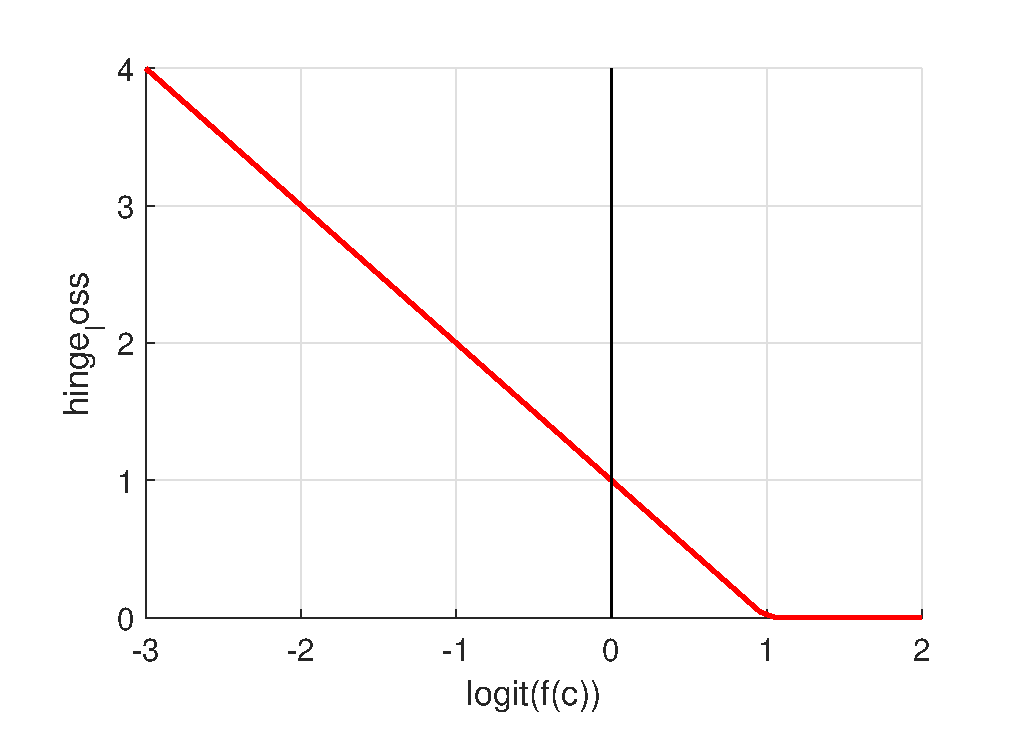
\includegraphics[width=0.5\textwidth]{hingeloss.eps}
  \caption{the hinge loss penalize wrong classification heavily, correct one near the boundary slightly and has no effect above a certain threshold}\label{fig:hingeloss}
\end{figure}

So far the equations are derived for a binary classification problem, where a ``why A not $\neg${A}'' or ``why A not B'' question is raised. For n-ary classification, where the prediction output is a n-length vector, \citeauthor{prototype} \cite{prototype} mentioned the following formula:
\begin{equation}\label{eq:lossPred}
  predloss=\max([f(\textbf{c})]_{i=i_0}-\max_{i\neq i_0}[f(\textbf{c})]_i),-\kappa)
\end{equation}
where $i_0=\arg\max f(\textbf{x})$ is the original data label, and $[f(\textbf{c})]_i$ is the i-th class prediction probability. This loss function gives a negative value if the predicted class is different than the original class, and $-\kappa < 0$ caps the negative value.

Now, equation \ref{eq:watcher} is already able to generate counterfactuals. However, it turns out that sometimes the given CF is hard to interpret and not actionable. Details of the issue are kept for section \ref{sec:adversarial}. To deal with the issue, some additional terms could be appended to the above equation to improve performance.

\subsubsection{add a diversity term}
As mentioned in the introduction, providing a diverse list of counterfactuals to choose from could be more helpful rather than one single "most feasible" solution. A valuable CF algorithm is able to generate multiple CF instances that are distinct from each other. Meanwhile, the counterfactuals should still proximate the original input. CFs that reach diversity by changes in numerous features, or too fierce changes, are considered inappropriate. This is realized by adding a specific diversity loss term to the loss function. \cite{DiCE} proposed to use the determinant of a kernel matrix as the diversity metric for n counterfactuals:
\begin{equation}\label{eq:dpp}
  dpp\_diversity(\mathbf{c_1,\dots,c_n})=\det(\mathbf{K}),\ \mathbf{K}_{i,j}=\frac{1}{1+dist(\mathbf{c_i,c_j})}
\end{equation}
%TODO: DPP的数学特征? OK
This matrix is named after a widely adopted sampling method DPP (determinantal point processes). DPP focuses on sampling diverse contents and avoiding redundancy. In DPP context the matrix shown above is referred as a marginal kernel. Note that marginal kernel is a mathematical definition, and this specific form is not the only way to construct it. A key rule is, the more similar the chosen candidates are, the smaller the determinant of the kernel matrix will be. For detailed mathematical derivation the readers are redirected to the second chapter of \cite{kulesza2011dpp}, here only an intuitional example is given.
\paragraph{dpp marginal kernel}
A DPP samples a subset \emph{A} of a discrete set \textbf{Y} with the following rule:
\begin{equation}\label{er:dpp}
  \mathcal{P}(A\subset\textbf{Y})=\det(K_A)
\end{equation}
which means the probability of choosing a certain subset equals to the minor of matrix \emph{K}, and \emph{K} is constructed by some relation of all elements in the complete set \textbf{Y}. Considering the simplest case with only two candidates \emph{i,j} in the subset, the possibility is:
\begin{equation}\label{eq:dpp1}
\begin{split}
  \mathcal{P}(i\in\textbf{Y})&=\det(K_{ii})=K_{ii}
\\
  \mathcal{P}(i,j\in\textbf{Y})&=\det\begin{pmatrix}
                                       K_{ii} & K_{ij} \\
                                       K_{ji} & K_{jj}
                                     \end{pmatrix}
                                      \\&=K_{ii}K_{jj}-K_{ij}K_{ji}
                                      \\&=\mathcal{P}(i\in\textbf{Y})\mathcal{P}(j\in\textbf{Y})-K_{ij}^2
\end{split}
\end{equation}
move a term to the left side we obtain the following equation, on the left side is exactly the definition of covariance:
\begin{equation}\label{eq:dpp2}
\begin{split}
  \mathcal{P}(i,j\in\textbf{Y})-\mathcal{P}(i\in\textbf{Y})\mathcal{P}(j\in\textbf{Y})=-K_{ij}^2
  \\\equiv Cov(i,j)=-K_{ij}^2
  \end{split}
\end{equation}
therefore, the possibility to choose a subset with two candidates equals the product of their independent possibility (marginal possibility) plus their (negative) covariance. The more relevant two candidates are, the higher $K_{ij}$ value is. When $\mathcal{P}(i),\mathcal{P}(j)$ are constants, a higher $K_{ij}$ value leads to a greater negative value of $\mathcal{P}(i,j)$ (i.e. the determinant of the matrix), which means a lower co-occurring chance. For 3-order matrix and higher, the explanation is no longer so intuitive.

Since multiple CFs are generated instead of only one, the basic formula needs to be modified before the diversity term is appended. The target loss and distance terms are averaged among all instances, a negative symbol is attached to diversity term because of the $\arg\min$ condition:
\begin{equation}\label{eq:DiCe}
\begin{split}
  \mathbf{C(x)}=\mathop{\arg\min}_{\mathbf{c_1,\dots,c_N}}&\frac{1}{N}\sum_{n=1}^{N}trgtloss(f(\mathbf{c_n}),y)
  +\frac{1}{N}\sum_{n=1}^{N}dist(\mathbf{c_n,x})
  \\&-dpp\_diversity(\mathbf{c_1,\dots,c_N})
\end{split}
\end{equation}
%TODO: Proximity, Sparsity 和Diversity的关系?
\subsubsection{add an interpretability term}
During the search of a CF example, it is equally important to demonstrate that the example is representable for the counter class, otherwise it is neither informative nor reasonable. For example, a user may want to change his occupation for better credits, but change the occupation to "professor" with educational background unchanged as "middle school" does not seem like a plausible answer. One trivial solution, as mentioned in the conclusion of \cite{bertossi2020asp}, is to abandon data generation, and only choose a closest case with the opposite label from a data bank.

To handle with this issue, \cite{prototype} proposed a prototype loss term, to measure the distance from the generated CF to other CF classes in latent layer. For each CF class \emph{i}, the algorithm firstly picks out the N nearest neighbours of the input that are classified as \emph{i}, then feeds them through an encoder and averages the output as the prototype of this CF class.
\begin{equation}\label{eq:prototype}
  proto_i=\frac{1}{N}\sum_{n=1}^{N}\mathbf{ENC}(\mathbf{x_n^i})
\end{equation}
Among all prototypes, the closest one to the input is chosen as the "guidance" for optimization:
\begin{equation}\label{eq:closestProto}
  j = {\arg\min}_{i\neq f(\textbf{x})}||\mathbf{ENC}(\textbf{x})-proto_i||_2
\end{equation}
The prototype loss term is defined as following:
\begin{equation}\label{eq:protoloss}
  prttyploss=||\mathbf{ENC}(\textbf{c})-proto_j||_2^2
\end{equation}
With the guidance of prototype, the perturbation is oriented to one chosen CF class rather than random search. The encoder used here could be any external known model, therefore requiring no internal information of the "black-box" model in question. We see that the closest target class to the input is chosen for a multiple classification task, this however could be revised for binary classification by explicitly choosing a target class.

\cite{prototype} furthermore shows that with the help of prototype loss term in searching, the target loss term could be dropped for improving efficiency. Generation methods based on loss function requires the gradient chain to know the optimization direction in next step. Unfortunately, as CF algorithms are often applied to "black-box" models, only the input data and the final prediction are available, the internal gradients are lost. Therefore, in order to measure the effect of a single perturbation of a feature \emph{k} on the final prediction, the gradient has to be approximated numerically by:
\begin{equation}\label{eq:gradientNumerical}
  \frac{\partial f_{pred}}{\partial x_k}\approx\frac{f_{pred}(x+\epsilon_k)-f_{pred}(x-\epsilon_k)}{2\epsilon}
\end{equation}
and this needs to be done on each feature in both directions for each gradient step, which results in numerous computation. For example, for a $28\times28$ MNIST image, the algorithm needs to call the model for $28\cdot28\cdot2$ times. Before, such numerous computation is still tolerated, because the target loss term ${trgtloss(f(\textbf{c}),y)}$ is the only roll that leads the generation to the target label. However, now the prototype loss term is also able to play the same guidance roll, and requires no internal information. The addition of ${prttyploss}$ significantly reduces both time and iterations about 80\%. Moreover, the generated CFs are more representative for one of the CF classes, as shown in figure \ref{fig:protoresult}. 
\begin{figure}
  \centering
  \includegraphics[width=0.5\textwidth]{proto.PNG}
  \caption{(a) column is the input data and (b) column is the CF output. In the first row, input class is 5 and CF class is 3. Second row, input class is 5 and CF class is 6. The addition of the prototype loss term generates a more interpretable CF.  
  }
  \label{fig:protoresult}
\end{figure}

The target loss term, in contrast, increases the time and results in a less interpretable CF, hence becomes a drawback in the whole formula and could be removed.
%\subsection{generation by replacing}
The loss function method in section \ref{sec:lossFunc} is mainly used for tabular data (\cite{DiCE,watcher2017,prototype}) or small image data (\cite{prototype}). For image data, even as small as MNIST, equation \ref{eq:watcher} turns out to be too expensive. Beside the prototype term, another way to generate an interpretable result for image data is to replace the identified region of an image with the identified region of one of its CF instances. \cite{visualCounterfactual} purposed the following formula:
\begin{equation}\label{eq:visualCF}
  h(I^\star)=(\mathbf{1}-\mathbf{a})\circ h(I)+\mathbf{a}\circ P\cdot h(I')
\end{equation}
where \emph{I} is the input image, and \emph{I'} is a chosen image with a different label. $h$ is a spatial feature extractor, so $h(I)\in\mathbb{R}^{hw\times d}$ is the mapped feature, where $h,w$ are the height and width of the image, and $d$ is the image dimension. $\circ$ is defined as the element-wise multiplication of the broadcasted vector (to match the size of a matrix) and the matrix. $\mathbf{a}\in\mathbb{R}^{hw}$ is a binary vector, with value of 1 indicates a substitution and 0 indicates not to substitute. \textbf{1} is a vector of all-ones, so \textbf{1-a} is the counterpart of \textbf{a}. $P\in\mathbb{R}^{hw\times hw}$ is a permutation matrix to rearrange elements of $h(I')$, so that the features of $h(I')$ align with $h(I)$.
%TODO: 什么是permutation matrix?
\paragraph{permutation matrix definition} A permutation matrix $P$ is a square binary matrix that has exactly one entry of 1 in each row and each column and 0s elsewhere. Multiplying $P$ with another matrix $A$ on the left shuffles the rows of $A$. A handy example is shown as follow:
$$
P=\begin{pmatrix}
    0 & 0 & 0 & 1 \\
    1 & 0 & 0 & 0 \\
    0 & 0 & 1 & 0 \\
    0 & 1 & 0 & 0
  \end{pmatrix},\
P\cdot\begin{pmatrix}
        1 \\
        2 \\
        3 \\
        4
      \end{pmatrix}=\begin{pmatrix}
                      4 \\
                      1 \\
                      3 \\
                      2
                    \end{pmatrix}
$$

By this replacing function, it is essential to minimize the replaced region to avoid the trivial solution of replacing the image with its CF  entirely. Since \textbf{a} is a binary vector, $||\textbf{a}||_1$ corresponds to the number of replaced pixels. The optimizing problem is equivalent to find a merged image classified as opposite label $i_c$ with minimum $||\textbf{a}||_1$:
\begin{equation}\label{eq:visualOpt}
\begin{split}
  \min_{P,\mathbf{a}} ||\mathbf{a}||_1
  \\s.t.\ &i_c=\arg\max f(h(I^\star))
  \\&a_i\in\{0,1\}\forall i,\ P\in \mathcal{P}
  \end{split}
\end{equation}
$f$ is a decision network to give out the final classification result of $I$, $f$ is assumed to be a multiple class classifier.

This task is still tremendously huge, because \textbf{a} is in $\mathbb{R}^{2^k}$ space and the permutation matrix is in $\mathbb{R}^{hw\times hw}$ space. It is equivalent to find a optimal subset of $hw*hw$ possible solutions. \cite{visualCounterfactual} used an exhaustive search approach to solve the problem. They break down the optimization to sequential steps. In each step, only one single spatial feature cell in $h(I')$ is chosen, and all permutation matrix will be probed to find the best location of this cell. The substitution is saved at the end of each step, steps are repeated until the modification is large enough to alter the prediction. The result is shown in figure \ref{fig:visualCF}.
\begin{figure}
  \centering
  \includegraphics[width=0.8\textwidth]{visualCFexample.PNG}
  \caption{In the first row, the permutation matrix mismatches two features and generates an incomprehensible result. In the second row, the features are aligned. 
  }\label{fig:visualCF}
\end{figure}

\subsection{Differential Evolution Method}
%The method in chapter \ref{sec:lossFunc} requires the objective function must be differentiable to evaluate the effect of perturbation on the final prediction.
Beside gradient descent, differential evolution (DE) or genetic method is another algorithm for solving optimization problems. DE is a population based optimization algorithm, its work principle could be briefly summarized as ``natural selection'' or ``survival of the fittest''. As the name implies, DE generates a new candidate set (children) from current set (parent), and only keep the candidates with the highest criteria (e.g. fitness value, diversity\dots) for the next iteration.

The prominent advantage of DE lies in three aspects: it is independent of whether the model is differentiable, and does not require internal gradients, this is the very case with a ``black-box'' model. Secondly, it is applicable for any sort of input data (continuous/categorical tabular data or image data). And finally, DE suffers less from local minima than gradient descent, partially due to the diversity in the candidate set.

The main steps of the genetic method is listed as follow \cite{certifai}:
\begin{enumerate}
  \item randomly generate points that belong to a CF class
  \item choose candidates with largest fitness value, where $fitness=\frac{1}{d(\textbf{x,c})}$
  \item mutate the candidates by arbitrarily changing their values
  \item randomly exchange some feature between candidates
\end{enumerate}
The steps are repeated until the maximum iteration is reached, and one single candidate with the best fitness is selected.

Similarly, another DE application of searching CF examples for image data is given by \citeauthor{onePixel} \cite{onePixel}. The result is impressive, see figure \ref{fig:onepixel}, because the CF has only one pixel changed compared to the original data. The evaluation formula as following:
\begin{equation}\label{eq:onepixel}
  \begin{split}
     &\max_{\mathbf c^\star} f_{i_c}(\mathbf{c})\\
     &subject\ to\ ||\mathbf{x-c}||_0=1
  \end{split}
\end{equation}
The formula maximize the prediction possibility of the target CF class $i_c$, while constraining the CF to be only one pixel different from the input. The 0-norm measures the number of non-zero elements, ensuring the sparsity.
\begin{figure}
  \centering
  \includegraphics[width=0.5\textwidth]{onepixel.PNG}
  \caption{one-pixel different CFs on CIFAR-10 dataset, a dataset that consists of $32\times32$ large images in 10 classes.
  The first row beneath each image is the original class, and the second row is the CF class. All three networks give out high confidence for the CF examples.}
  \label{fig:onepixel}
\end{figure}


\subsection{Summary of Nearest Counterfactual Method}
%移动到第一章结尾
Here we summarize the metrics that nearest CF explanation is able to fulfill.
 \begin{itemize}
 \item Validity: CF is classified in the desired class.
 \item Proximity: CF is similar to the input data point.
   \item  Sparsity: CF should prescribe a small change in a small number of features because shorter explanations are more comprehensible to humans \cite{CFReview}. %This is done by \emph{L1} norm in gradient-based method and {L0} in genetic method.
   \item  Diversity: multiple CFs for one input. CFs should have maximum distance between each other, while each of them keep proximate to the input.
   \item  Training Data Distribution: CF should be representative for its class, leaving human an impression that it is correctly classified.
 \end{itemize} 
\section{Drawbacks of Nearest Counterfactual Explanation}\label{sec:adversarial}

\subsection{Shadow of Adversarial Examples}
It is observed that the examples generated by the genetic method are too close to the input that their new classification result seems not convincing \cite{onePixel,certifai}. Though the CF gives out a different prediction result, it still falls in the original class out of the human perspective, indicating that it is classified incorrectly. And except for the prototype variation, other gradient-based methods also suffer from this issue \cite{prototype}. Such examples that are almost identical to the original input but successfully ``fooled'' the model is another research topic called ``adversarial examples'' (AE). \autoref{fig:AE} shows a model can be fooled by a randomly generated rubbish pattern. The aim of AE is to deceive the system, while the aim of CF is to give a plausible counter-instance.

The difference between AE and CF is obscure. Because popular algorithms to generate an AE are also gradient-based methods or genetic methods \cite{AEoverview}. Both of them pursue a different prediction with small perturbation to the input data. CFs and AEs to some extent share the same mathematical framework and are sometimes inter-transferable \cite{CFandAE}. The main differences lie in two aspects:
\begin{itemize}
  \item Prediction Result: the key criterion is whether the prediction is correct. Examples generated by adversarial algorithms are \emph{misclassified}, while examples generated by counterfactual explanations are correctly classified. Whether a classification is correct or not, is left to a human's judgement.
  \item Perturbation: the standard perturbation for AEs is adding a subtle global noise to the image. The hidden perturbation should be imperceptible to human eyes but is sufficient to mislead the model. In contrast for CF explanations, while keeping sparsity of the explanation, the perturbation is the key for understanding and should be highlighted.  %TODO: 这里缺张图
\end{itemize}
\begin{figure}
  \centering
  \includegraphics[width=0.7\textwidth]{adversarial.PNG}
  \caption{An example of AE: after adding a rubbish pattern to the original image, the model gives out another prediction with extremely high confidence. Credit: \cite{goodfellow2014explaining}}
  \label{fig:AE}
\end{figure}

By generating CFs, how do we avoid  ``gaming'' the system like the AEs? At first glance, it is impossible to distinguish them in practice because their mathematical principles are almost the same. Both required a different prediction result, and both need the perturbation to be small. But fortunately, there is one way out, which is the definition of ``near''. AEs need a perturbed input that is near to the original one because the perturbation should be not noticeable, while CFs need a near input so that the user is able to comprehend the main difference. In the case of CFs, the minimality of perturbation is not as important as for AEs, and it is enough to find inputs close enough to the original input that changes the classification in the desired way \cite{CFandAE}. The nearest CF explanations introduced in section \ref{sec:generation} are able to find CFs that are \emph{semantically} meaningful in distance function between different examples, but their benefits to the users are questionable.

Are nearest CF explanations wrong? Actually, ``counterfactual explanation'' is a broad topic, under which fall at least two groups of literature. Let's recap the two basic requirements of CFs here: a CF is a close input to the original input with a different prediction, i.e. equation \ref{eq:watcher}. Some authors develop their method under this assumption (e.g. \cite{certifai,watcher2017,DiCE}), and don't mention how to distinguish CFs generated by their purposed methods from AEs. Meanwhile, other authors expected more under this topic (e.g. \cite{prototype}), and they develop methods that prefer ``feasible'' solutions. Both groups, however, are a part of the big topic. Even though the latter sounds more favorable to a user, it is hard to exclude the former out of CF explanations. \citeauthor{CFandAE} \cite{CFandAE} has divided CF methods into two categories, namely \emph{contesting CF} and \emph{feasible CF}. The author argues that while the feasible CFs are useful in providing the user an actionable solution, the contesting CFs are useful in contesting a decision and therefore are similar to AEs. The author also clarifies the common misconceptions, pointing out that CFs are not equal to AEs, and feasible CFs are not all about CF explanation. In one word, $AE\approx contesting\ CF\subseteq CF$.
 \subsection{Lack of Actionability}
Consider the loan lending example again, an explanation may be ``You will be offered the loan if you decrease your age by three and change the education level to master.'' This explanation is certainly plausible (the bank system has seen someone who is younger but with a higher degree), but not actionable because the user could do nothing to improve his situation. A common criticism of nearest CF explanation methods is that they only answer the question of \emph{``what could have been done in the past''}, while the original aim of CF explanation should be \emph{``what should be done in the future''} \cite{algorithmicrecourse}.

There is a general agreement that causal constraints need to be taken into consideration for a feasible CF \cite{algorithmicrecourse}. Specifically, these constraints may include but are not limited to:
 \begin{itemize}
   \item Unary Causality Constraints: for example, age can not decrease with time.
   \item Binary Causality Constraints: other notations of this term are feature correlation \cite{preservingCausal} or downstream effects \cite{algorithmicrecourse}. For example changing the education level without an increase in age is not possible \cite{DiCE}.
   \item True Causality Connection: avoid spurious connections between a feature with the final prediction. For example, the higher salary one earns, the more dogs he can afford. But for loan approval the salary should be the only deciding feature, the model should not suggest a solution like ``if you raise one more dog, you will be offered with the loan'' \cite{diffThatMakesDiff}.
 \end{itemize}

What's more, it is worth mentioning that each CF is unique and user-specific. Besides the causal constraints, there may be also user-defined constraints, which the user is able to do but not willing to do, for example changing the city \cite{preservingCausal}. However, for the following discussion, these constraints are excluded to lay the main focus on causality.

%If these additional requirements are not fulfilled, the explanation can not be distinguished from an AE clearly and easily leaves an impression of deceiving the model. However, these additional requirements are rarely satisfied by the nearest CF methods. \cite{DiCE} has used a post-hoc filter to pick out the feasible explanations, but this is not the optimal solution. To generate feasible CFs, there is a general agreement that causal models, namely the effect of changing a variable on other variables, is a promising way out \cite{algorithmicrecourse}.

%%Nearest explanation answers the question ``what could have been done'', while casualty explanation answers ``what to do now'' 
\section{Causality model}\label{sec:Causality}
\section{Conclusion}\label{sec:Conclude}
% ---- Bibliography ----
%
% BibTeX users should specify bibliography style 'splncs04'.
% References will then be sorted and formatted in the correct style.
%
% \bibliographystyle{splncs04}
% \bibliography{mybibliography}
%
\bibliographystyle{plainnat}
%\bibliographystyle{splncs04}
\bibliography{Reference}{}
\end{document}
